%  Copyright 2020-2026 Robert Bosch GmbH
%
%  Licensed under the Apache License, Version 2.0 (the "License");
%  you may not use this file except in compliance with the License.
%  You may obtain a copy of the License at
%
%      http://www.apache.org/licenses/LICENSE-2.0
%
%  Unless required by applicable law or agreed to in writing, software
%  distributed under the License is distributed on an "AS IS" BASIS,
%  WITHOUT WARRANTIES OR CONDITIONS OF ANY KIND, either express or implied.
%  See the License for the specific language governing permissions and
%  limitations under the License.

\section{Introduction}
Roo Code is an autonomous AI software engineer that operates directly within
the VSCodium.
Unlike standard AI assistants, Roo Code can interact with your file system,
execute terminal commands, and use a browser to provide a seamless,
agentic development experience.

\section{Installation}
Roo Code Extension is pre-installed in the \textbf{Robot Framework AIO} package.

You can find it in the \textbf{Activity Bar} as the \textbf{Roo Code} icon or
in the \textbf{Extensions} view as below:

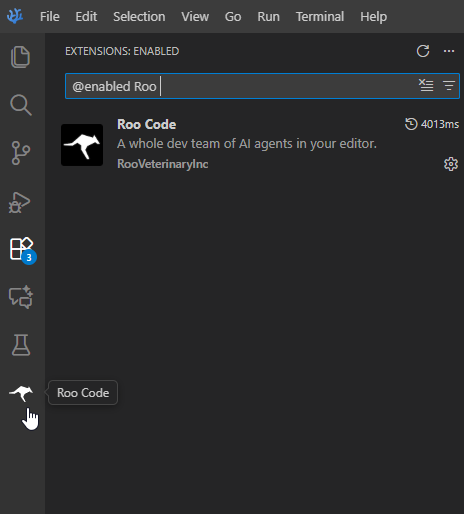
\includegraphics{./include/graphics/roocode/RooCodeExtension.png}

\section{Key Features}
Roo Code enhances the development experience in
\textbf{VSCodium For RobotFramework} with several "agentic" capabilities:
\begin{itemize}
   \item \textbf{Autonomous Coding:}
      Reads, writes, and creates files based on natural language.
   \item \textbf{Terminal Control:}
      Executes shell commands (e.g., running Robot Framework tests,
      installing pip packages) and self-fixes based on output.
   \item \textbf{Self-Healing Tests:}
      Automatically analyzes test failures and refactors code until tests pass.
   \item \textbf{Browser Integration:}
      Launches a headless browser to inspect UIs or gather documentation.
   \item \textbf{MCP Support:}
      Connects to external tools (Google Drive, GitHub, Slack) via the
      Model Context Protocol - MCP.
\end{itemize}
